\documentclass[11pt, letterpaper, twoside]{article}
\usepackage[letterpaper, portrait, left=1in, right=1in, top=1in, bottom=1in]{geometry}\usepackage{amsmath}
\usepackage{amssymb}
\usepackage{graphicx}
\usepackage[explicit]{titlesec}
\usepackage{epstopdf}
\usepackage{amsmath}
\usepackage{inputenc}
\usepackage{enumitem}
\usepackage{booktabs, multirow} %for borders and merged ranges
\usepackage{soul}% for underlines
\usepackage[table]{xcolor} % for cell colors
\newcommand\aug{\fboxsep=-\fboxrule\!\!\!\fbox{\strut}\!\!\!} %Use \aug to make a equal column for an augmented matrix. Ie. 1 & 2 & 3 & 4 & \aug & x \\
\begin{document}
\begin{titlepage}
\centering
\vspace*{60px}
\hspace{0pt}

\includegraphics[width=0.2\textwidth]{logo}\par\vspace{1cm}
{\scshape\LARGE Athabasca University \par}
\vspace{1cm}
{\scshape\Large MATH 265\par}
\vspace{1.5cm}
{\huge\bfseries Assignment 4\par}
\vspace{2cm}
{\Large\itshape Stanley Zheng\par}
\vfill
{\large September 3, 2020\par}
\vspace*{50px}
\hspace{0pt}
\pagebreak
\end{titlepage}
\begin{enumerate}
\item 
\begin{enumerate}[label=\alph*)]
\item ‌‌ 

\vspace{0.2cm}
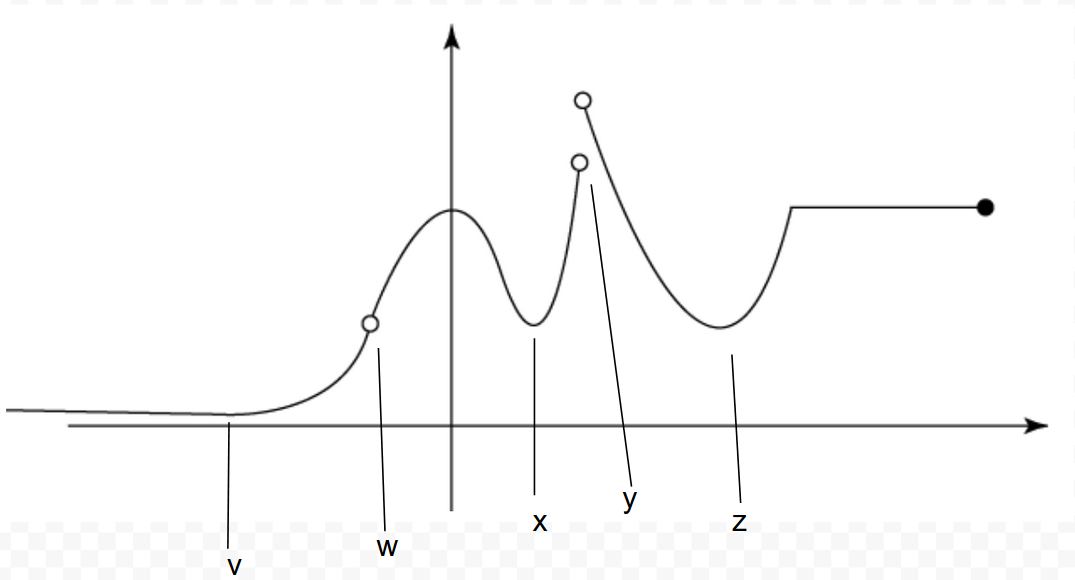
\includegraphics[width=0.7\textwidth]{q1}\par

The domain of the function \(g\) is \((-\infty, w)\cup(w, x)\cup(x, y]\)
\item The function \(g\) is continuous from \((-\infty, w)\cup(w, x)\cup(x, y]\).
\item The local maximum ix at \(x=0\), since the derivative is 0.
\item The local minimum is at two points, \(x\) and \(z\), where the derivative is zero.
\item There is no absolute maximum as the derivative at \(y\) is undefined, and \(y\) is not included in the domain.
\item The absolute minimum is at \(v\). It appears as though the graph has negative slope as \(x\) decreases beyond \(v\) to infinity.
\end{enumerate}
\item %q2



\item %q3
\end{enumerate}
\end{document}
